%%\documentclass[hyperref={pdfpagelabels=false},compress]{beamer}
\documentclass[10pt]{beamer}

\usetheme{default}
%\usetheme{metropolis}
\useoutertheme{noslidenum}
\usefonttheme[onlylarge]{serif}
% \usecolortheme{beaver}
\usecolortheme{UCLAsquirrel}
%\logo{\includegraphics[height=0.7cm]{/home/sudiptob/texmf/tex/latex/uclabeamer/logo_ucla_cw.png}}

\setbeamerfont*{frametitle}{size=\normalsize,series=\bfseries}
\setbeamertemplate{navigation symbols}{}

\usepackage{lmodern}
%\usepackage{subfigure}
\usepackage{subfig}
\usepackage{pifont}
\usepackage{tabu}
\usepackage{xcolor}
\usepackage{algorithm}
\usepackage{algpseudocode}
%\usepackage{enumitem}
\usepackage{remreset}
\usepackage{etoolbox}
\usepackage{comment} % end and begin comment
%\usepackage{dtklogos} 
\usepackage{listings}
\lstset{breaklines=true} 
\usepackage{cancel}
\usepackage{epstopdf}
\usepackage{overpic}
\usepackage{url}
\usepackage{calrsfs}
\usepackage{mathrsfs}
\usepackage{epsfig}
\usepackage{cancel}
\usepackage{changepage}

\usepackage[english]{babel}
\usepackage[latin1]{inputenc}
\usepackage{times}
\usepackage[T1]{fontenc}
\usepackage{tikz}
\usetikzlibrary{arrows}
\tikzstyle{block}=[draw opacity=0.7,line width=1.4cm]
\let\code=\texttt
\let\proglang=\textsf

\newcommand{\gline}{\textcolor{gray}{\hline}}
\newcommand{\cmark}{\ding{51}}%
\newcommand{\xmark}{\ding{55}}%
\newcommand{\gcheck}{\textcolor{blue}{\Large \cmark}}
\newcommand{\rcross}{\textcolor{red}{\Large \xmark}}
\newcommand{\tkt}{\tilde{K}_\theta}
\newcommand{\kt}{K_\theta}
\newcommand{\ind}{\overset{ind}{\sim}}
\newcommand{\plim}{\overset{p}{\rightarrow}}
\newcommand{\cx}{\frac {X'X}n}
\newcommand{\cz}{\frac {Z'Z}n}
\newcommand{\ccz}{\frac {Z'Z}n - \Sigma_A}
\newcommand{\czy}{\frac {Z'y}n}
\newcommand{\cyz}{\frac {y'Z}n}
\newcommand{\cxy}{\frac {X'y}n}
\newcommand{\cyx}{\frac {y'X}n}
\newcommand{\myitem}{\vskip3mm \item}
%\newcommand{\iid}{\overset{iid}{\sim}}

\newcommand{\calS}{{\cal S}}
\newcommand{\calA}{{\cal A}}
\newcommand{\calK}{{\cal K}}
\newcommand{\calX}{{\cal X}}
\newcommand{\calD}{{\cal D}}
\newcommand{\calG}{{\cal G}}
\newcommand{\calT}{{\cal T}}
\newcommand{\calU}{{\cal U}}
\newcommand{\calR}{{\cal R}}
\newcommand{\tp}{\tilde{p}}
\newcommand{\tildebC}{\tilde{\bC}}
\newcommand{\calL}{{\cal L}}
\newcommand{\calP}{{\cal P}}

\newcommand{\given}{\, | \,}


%\newcommand{\T}{\top}

\newcommand{\blue}[1]{{\color{RoyalBlue!90} #1}}
\newcommand{\red}[1]{{\color{Red} #1}}
\newcommand{\green}[1]{{\color{Green} #1}}
\newcommand{\titl}[1]{{\begin{large}\begin{center}#1\end{center}\end{large}}}

\title[BIOSTAT~241] 
{%
CAR: Conditional Auto-Regression Models
}

\author[Sudipto Banerjee]
{
 Sudipto Banerjee
}

\institute[UCLA]
{
  University of California, Los Angeles, USA
}

\date[]{}

\begin{document}
\begin{frame}
 \titlepage
\end{frame}

\begin{frame}{Simple linear regression: continuous outcomes}

\begin{itemize}
 \item Units: $i=1,2,\ldots,n$; Outcome: $y_i$; Predictor: $x_i$

 \item Recall simple linear regression:
\[
 y_i = \beta_0 + \beta_1 x_i + \epsilon_i\;;\quad i=1,2,\ldots n 
\]
 
 \item Multiple linear regression:
\[
 y_i = \beta_0 + \beta_1 x_{1i} + \beta_2 x_{2i} + \cdots + \beta_p x_{pi} + \epsilon_i\;;\quad i=1,2,\ldots n 
\] 

 \item The errors: $\epsilon_i \stackrel{iid}{\sim} N(0,\sigma^2)$:
 \begin{align*}
  y_i \given \mu_i,\: \sigma^2 &\stackrel{ind}{\sim} N(\mu_i, \sigma^2)\;; \\
  \mu_i &= \beta_0 + \beta_1 x_{1i} + \beta_2 x_{2i} + \cdots + \beta_p x_{pi}\;. 
 \end{align*}

 \item  How do we estimate the regression coefficients and the residual variance $\sigma^2$. 
\end{itemize}

% \[
%  [\mbox{data} \given \mbox{parameters}, \mbox{random effects}] \times [\mbox{random effects} \given \mbox{parameters}] \times [\mbox{parameters}]
% \]

\end{frame}

\begin{frame}{Bayesian Hierarchical Models}
 
 \begin{multline*}
  y_i \given \mu_i,\: \sigma^2 \stackrel{ind}{\sim} N(\mu_i, \sigma^2)\;;\quad i=1,2,\ldots,n\;; \\
  \mu_i = \beta_0 + \beta_1 x_{1i} + \beta_2 x_{2i} + \cdots + \beta_p x_{pi}\;;\quad i=1,2,\ldots,n\;; \\
  \beta_j \stackrel{ind}{\sim} N(0, \sigma^2_{\beta})\;;\quad j=0,1,\ldots,p\;; 1/\sigma^2 \sim \mbox{Gamma}(a,b)\;. 
 \end{multline*}
 
\end{frame}


\begin{frame}{Bayesian Generalized linear models}
 
 \begin{itemize}
  \item Binary data:
  \begin{multline*}
   y_i \sim Ber(p_i)\;;\quad i=1,2,\ldots,n\;;\\
   \log\frac{p_i}{1-p_i} = \beta_0 + \beta_1 x_{1i} + \beta_2 x_{2i} + \cdots + \beta_p x_{pi}\;;\quad i=1,2,\ldots,n\;; \\
   \beta_j \stackrel{ind}{\sim} N(0, \sigma^2_{\beta})\;; \quad j=0,1,\ldots,p\;. 
  \end{multline*}

  \item Count data:
  \begin{multline*}
   y_i \sim Poi(\lambda_i)\;;\quad i=1,2,\ldots,n\;;\\
   \log\lambda_i = \beta_0 + \beta_1 x_{1i} + \beta_2 x_{2i} + \cdots + \beta_p x_{pi}\;;\quad i=1,2,\ldots,n\;; \\
   \beta_j \stackrel{ind}{\sim} N(0, \sigma^2_{\beta})\;; \quad j=0,1,\ldots,p\;. 
  \end{multline*}
  
 \end{itemize}

\end{frame}

\begin{frame}{Random effect models}
 
 \begin{itemize}
  \item Continuous data:
   \begin{multline*}
  y_i \given \mu_i,\: \sigma^2 \stackrel{ind}{\sim} N(\mu_i, \sigma^2)\;;\quad i=1,2,\ldots,n\;; \\
  \mu_i = \beta_0 + \beta_1 x_{1i} + \beta_2 x_{2i} + \cdots + \beta_p x_{pi} + w_i\;;\quad i=1,2,\ldots,n\;; \\
  \beta_j \stackrel{ind}{\sim} N(0, \sigma^2_{\beta})\;;\quad j=0,1,\ldots,p\;; \\ 
  w = (w_1, w_2,\ldots, w_n)^{\top} \sim N(0,V_w)\;;\quad 1/\sigma^2 \sim \mbox{Gamma}(a,b)\;.
 \end{multline*}
 
 \item Count data:
 \begin{multline*}
   y_i \sim Poi(\lambda_i)\;;\quad i=1,2,\ldots,n\;;\\
   \log\lambda_i = \beta_0 + \beta_1 x_{1i} + \beta_2 x_{2i} + \cdots + \beta_p x_{pi} + w_i\;;\quad i=1,2,\ldots,n\;; \\
   \beta_j \stackrel{ind}{\sim} N(0, \sigma^2_{\beta})\;; \quad j=0,1,\ldots,p\;;\quad w \sim N(0,V_w)\;.  
  \end{multline*}
 
 \item $V_w$ introduce dependence among $w_i$'s---and among $y_i$'s. 
 \end{itemize}

\end{frame}


\begin{frame}{Toward spatial dependence: Adjacency or proximity matrices}
\begin{itemize}\setlength{\itemsep}{0.3cm}
\item $A$, entries $a_{ij}$, ($a_{ii}=0$); choices for $a_{ij}$:

\begin{itemize}
\item
$a_{ij}=1$ if $i,j$ share a common boundary (possibly
a common vertex)
\item
$a_{ij}$ is an \emph{inverse} distance
between units
\item
$a_{ij}=1$ if distance between units is $\le K$
\item
$a_{ij}=1$ for m nearest neighbors.
\end{itemize}

\item $A$ need not be symmetric.

\item $\widetilde{A}$:   standardize row $i$ by $a_{i+}= \sum_{j}
a_{ij}$ (row stochastic but need not be symmetric).

\item $A$ elements often called ``weights''; perhaps nicer interpretation?

\end{itemize} 
\end{frame}

\begin{frame}{CAR models}
	\begin{itemize}
		\item CAR model:
		\begin{equation*}
		w_i \given w_{-i} \sim N\left(\frac{\rho\sum_{j} a_{ij} w_j}{\sum_{j}a_{ij}}, \frac{\sigma_w^2}{\sum_{j} a_{ij}} \right)
		\end{equation*}
		\item Joint density for $w$: $w=(w_1,w_2,\ldots,w_n)^{\top} \sim N(0, V_w)$ 
		\myitem $V_w^{-1} = \left(1/\sigma_w^2\right) (D-\rho A)$; $D=\mbox{diag}\left(\sum_{j}a_{1j}, \sum_{j}a_{2j}, \ldots, \sum_{j}a_{nj}\right)$.
		\myitem Usual specification: $a_{ii}=0$ and $a_{ij} = I(i \leftrightarrow j)$.
		\only<1>{\myitem $\rho = 1 \Rightarrow$ Improper distribution as $(D-A)1 = 0$ \alert{(ICAR)}
		\begin{itemize}
		\item Can be used as a prior for random effects
		\item Cannot be used directly as a data generating model
		\end{itemize}}
		\only<1>{\myitem $\rho <1 \Rightarrow$ Proper distribution with added parameter flexibility}		
		%\myitem Often oversmooth spatial random effects
	\end{itemize}
\end{frame}

\begin{frame}{Disease Mapping: Mapping Random Effects}

%Model-based estimates of random effects across $87$ counties in Minnesota

{\tiny
\begin{align*}
 \mbox{[Infant Mortality Rates]} &= \mbox{[Intercept]} + \mbox{[Fixed Effects]} + \mbox{[County-wise Random Effects]}
\end{align*}
}

\vspace{-0.25in}
\begin{center}
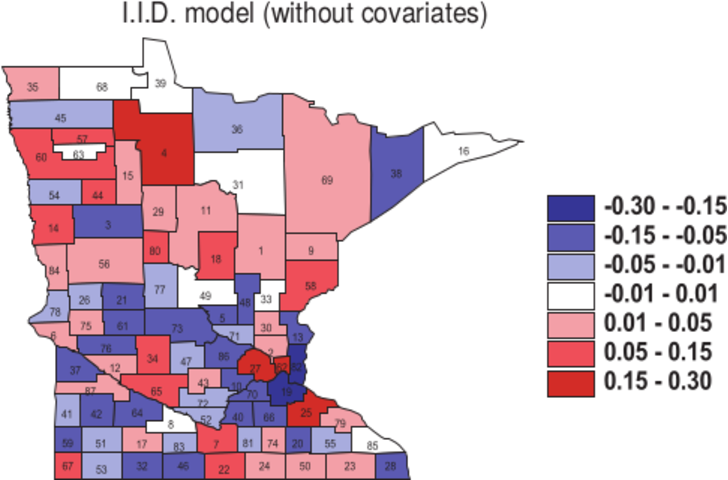
\includegraphics[width=0.35\textwidth, height=0.35\textheight]{figs/BWC_IID_Without_Covariates}
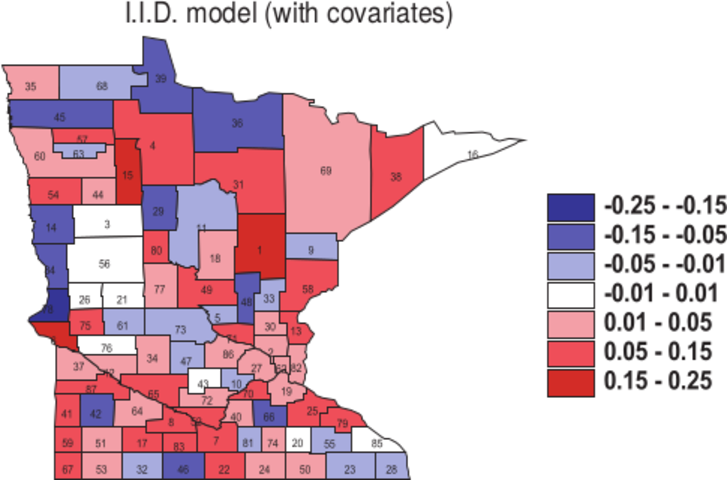
\includegraphics[width=0.35\textwidth, height=0.35\textheight]{figs/BWC_IID_With_Covariates}\\
\vspace{0.15in}
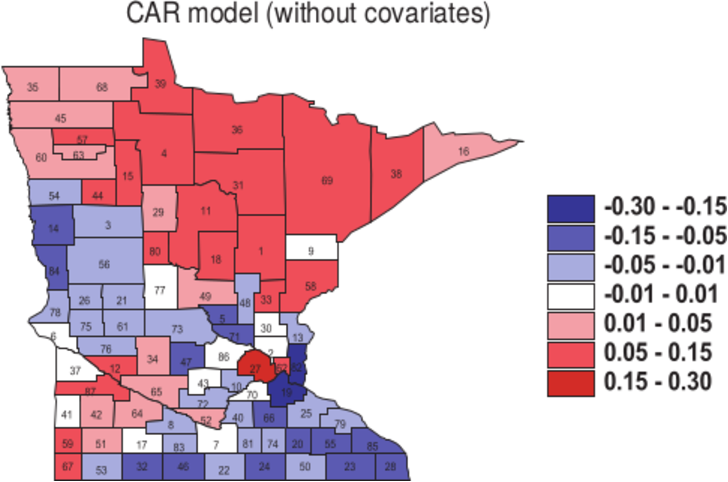
\includegraphics[width=0.35\textwidth, height=0.35\textheight]{figs/BWC_CAR_Without_Covariates}
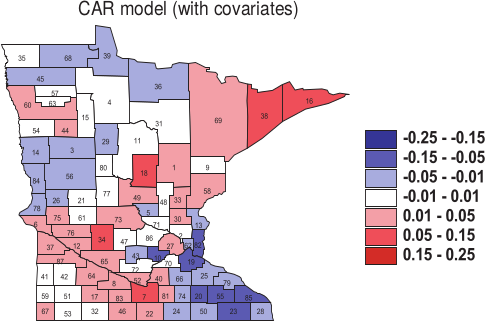
\includegraphics[width=0.35\textwidth, height=0.35\textheight]{figs/BWC_CAR_With_Covariates}
\end{center}

\end{frame}

\begin{frame}{Other versions of CAR models}

\begin{itemize}
 \item Besag-York-Mollie (BYM):
 \begin{equation*}
 \begin{split}
  \mu_i &= \beta_0 + \beta_1 x_{1i} + \beta_2 x_{2i} + \cdots + \beta_p x_{pi} + w_i + v_i\;; \\
  w_i \given w_{-i} &\sim N\left(\frac{\sum_{j} a_{ij} w_j}{\sum_{j}a_{ij}}, \frac{\sigma_w^2}{\sum_{j} a_{ij}} \right)\;;\quad v_i \sim N(0,\sigma_v^2)\;. 
 \end{split}
 \end{equation*}

 \item Leroux et al. (2000) proposed the following alternative CAR prior for modeling varying strengths of spatial autocorrelation using only a single set of random effects:
 \begin{equation*}
		w_i \given w_{-i} \sim N\left(\frac{\rho\sum_{j} a_{ij} w_j}{\rho\sum_{j} a_{ij} + 1 - \rho}, \frac{\sigma^2}{\rho \sum_{j} a_{ij} + 1 - \rho}\right)
		\end{equation*}
\end{itemize}

\end{frame}

\end{document}
